\documentclass[12pt]{article}

\usepackage{amsmath, amssymb, amsfonts}
\usepackage{fullpage}
\usepackage{graphicx}
\usepackage{listings}
\usepackage{refcount}
\usepackage{hyperref}
\usepackage{float}

\usepackage{color}

\definecolor{codegreen}{rgb}{0,0.6,0}
\definecolor{codegray}{rgb}{0.5,0.5,0.5}
\definecolor{codepurple}{rgb}{0.58,0,0.82}
\definecolor{backcolour}{rgb}{0.95,0.95,0.92}

\lstdefinestyle{mystyle}{
    backgroundcolor=\color{backcolour},   
    commentstyle=\color{codegreen},
    keywordstyle=\color{magenta},
    numberstyle=\tiny\color{codegray},
    stringstyle=\color{codepurple},
    basicstyle=\footnotesize\ttfamily,
    breakatwhitespace=false,         
    breaklines=true,                 
    captionpos=b,                    
    keepspaces=true,                 
    numbers=left,                    
    numbersep=5pt,                  
    showspaces=false,                
    showstringspaces=false,
    showtabs=false,                  
    tabsize=2
}

\lstset{style=mystyle}


\title{\huge From Biology to Computation: Exploring Genetic Algorithms}
\author{\href{samaniloqman91@gmail.com}{Loghman Samani}}
\date{\today}

\begin{document}

\maketitle

\newpage

\tableofcontents

\newpage

\section{Introduction}

Genetic algorithms are a family of optimization algorithms inspired by natural evolution. These algorithms simulate the process of evolving solutions to problems, using biological concepts like selection, crossover, and mutation through generations or iterations. In this article, we will start by explaining biological evolution, its mechanisms, and the concepts fundamental to genetic algorithms, step by step. Then, we will go through the genetic algorithm itself, explaining each concept and implementing it in Python. Furthermore, we will use the Python code to solve some optimization problems and analyze the results.\\[6px]

\section{Biological Basis of Genetic Algorithms}

Our world is full of diverse entities, from living organisms to inanimate objects, all interconnected through various relationships. Among these, the relationships and hierarchy within the living world, including viruses, are particularly fascinating. Evolution is a key concept that explains this complexity. The theory of evolution by natural selection describes how species evolve and adapt over time.

In this section, we will explore the fundamental concepts of evolution, focusing on biological and molecular biology ideas, and explain how these concepts form the basis of genetic algorithms.\\[6px]


\subsection{Theory of Evolution by Natural Selection}

In 1858, Charles Darwin and Alfred Russel Wallace independently proposed natural selection as the main mechanism responsible for generating new phenotypes and ultimately new species. This mechanism serves as the basic explanation for the evolution of living organisms. The proposed mechanism makes five fundamental assertions:\\[5px]

    - Organisms typically have more offspring than their environment can sustain.

    - Within a species, there is a wide range of differences in various traits among individuals.

    - Individuals of a species compete for limited resources in their environment.

    - Traits inherited from parents can change over generations.

    - Over time, these changes can lead to the emergence of new species.\\[5px]

Although many questions in evolutionary biology remain, no credible scientist denies evolution as a fact. The mechanism of evolution, which relies on natural selection as proposed by Darwin and Wallace, has been modified and adapted over the years. New concepts from various branches of biology, such as molecular genetics, physiology, systems biology, and others, have contributed to this evolving understanding.

Today, scientists continue to refine the mechanisms explaining how evolution works. The objective is to explain how new species are produced and what drives diversity within populations. Natural selection is seen as a powerful tool that eliminates individuals who are not well-adapted to their environment. The origin of diversity, enhanced by advances in molecular biology, is explained by processes like crossover and mutation. Crossover occurs intracellularly in organisms with sex organs (those producing gametes through meiosis) and introduces genetic diversity. Mutations, which often have extracellular sources, also contribute to the genetic variation within a population.

\subsection{Genes and Chromosomes}

When we talk about the diversity changes in a population, we often think of visible traits, but from a biological perspective, these visible traits, known as phenotypes, are less important. Modern evolutionary biology explains natural selection at the molecular level using concepts like genes, chromosomes, crossover, mutation, and genotype. Each of these concepts plays a crucial role in understanding the mechanism of natural selection.

Each cell in our body contains a nucleus (with some exceptions like red blood cells), where genetic information is stored and protected. This genetic information is divided into different parts, each called a chromosome. In humans, there are 23 pairs of chromosomes (Figure 1). Each chromosome contains a set of genes. For example, a small chromosome like chromosome 21 contains about 300-400 genes, while a large chromosome like chromosome 1 contains 4000-4300 genes (figure 2). Each gene occupies a specific location on the chromosome called a locus.

During fertilization, humans inherit a set of 23 chromosomes from each parent. Each pair of chromosomes contains different versions of a gene, inherited from different parents.\\[6px]

\begin{figure}[H] 
\centering 
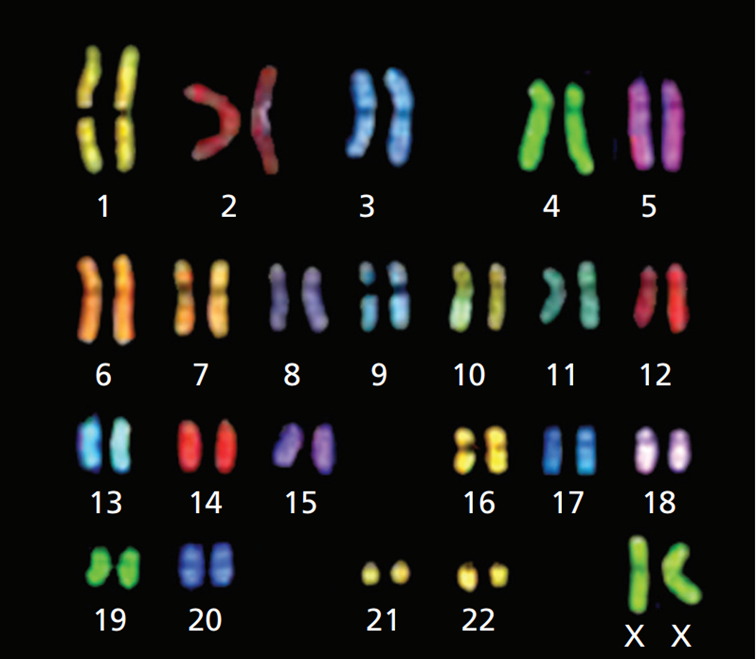
\includegraphics[scale=0.75]{Picture1}\\
\caption{The complete set of human chromosomes. (Alberts, B. (seventh edition). Molecular Biology of the Cell
)}
\end{figure} 

\begin{figure}[H]
\centering
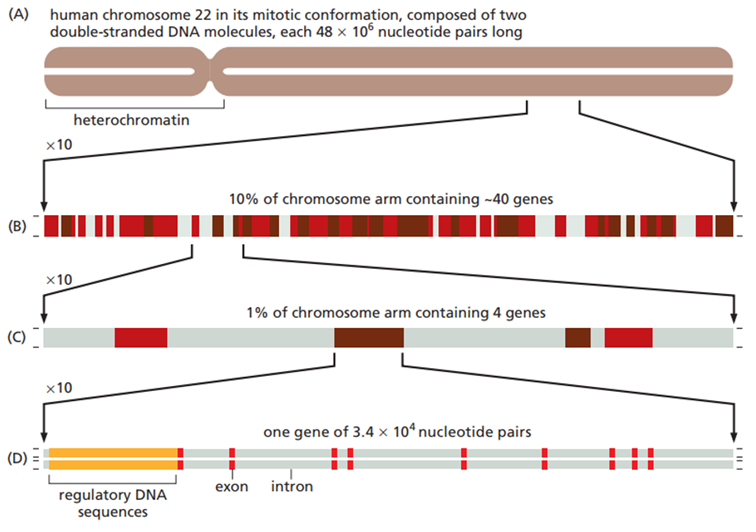
\includegraphics[scale=0.85]{Picture2}\\
\caption{The organization of genes on a human chromosome, as determined from the initial sequencing of the human genome.(Alberts, B. (seventh edition). Molecular Biology of the Cell
)}
\end{figure}


\subsection{Biological Recombination}

In most eukaryotic organisms, the process of generating offspring is sexual, meaning two parents are required. Their genomes mix to produce offspring that are generally distinct from both parents. Each cell in the offspring (or any eukaryotic organism) contains two sets of chromosomes, one from each parent. During fertilization, these sets must be reduced to one set, which is achieved through a specific type of cell division called meiosis.

In the early stages of meiosis, particularly during prophase I, a process called recombination occurs. This is when genetic information is exchanged between two homologous chromosomes, contributing significantly to the diversity of the population. During recombination, DNA double-strand breaks form at several locations in each sister chromatid, resulting in numerous DNA recombination events between the homologs. Some of these events lead to reciprocal DNA exchanges called crossovers, where the DNA of one chromatid crosses over to become continuous with the DNA of a homologous chromatid (figure 3).

Recombination is one of the key reasons for genetic diversity, ensuring that offspring have unique combinations of traits inherited from their parents.\\[6px]


\begin{figure}[H]
\centering
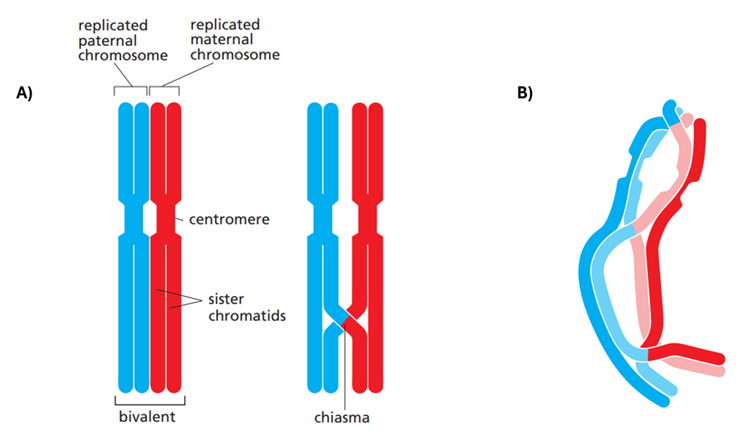
\includegraphics[scale=1]{Picture3}\\
\caption{Homolog pairing and crossing-over. A) A bivalent in which a
single crossover has occurred between nonsister chromatids: B) A bivalent with three chiasmata resulting from three crossover events. (Alberts, B. (seventh edition). Molecular Biology of the Cell
)}
\end{figure}



\subsection{Biological Mutation}

A biological mutation is a change in the building blocks of DNA, which are nucleotides. Nucleotides are composed of three molecules: nitrogen-containing bases (guanine, adenine, cytosine, and thymine), deoxyribose (sugar), and phosphate (figure 4). Mutations can be caused by various sources, from internal mistakes that occur during DNA replication to external factors like specific chemicals and radiation.

There are four major types of mutations: substitution, deletion, insertion, and inversion (figure 5). Each type can occur at different phases of an organism's life and can have different consequences. 

    \textbf{1. Substitution Mutation:} A base or sometimes a part of DNA (more than one base) is replaced by another base. For example, an adenine (A) might be replaced with a guanine (G).

    \textbf{2. Insertion Mutation:} One or more bases are added to a DNA sequence. 

    \textbf{3. Deletion Mutation:} A base or a part of DNA is removed, resulting in the loss of genetic information.

    \textbf{4. Inversion Mutation:} A part of DNA is cut out and reattached to the same location but in reverse order.

Each type of mutation can have various effects on the organism, ranging from no noticeable impact to significant changes in phenotype, potentially leading to evolutionary advantages or disadvantages.\\[6px]

 

\begin{figure}[H]
\centering
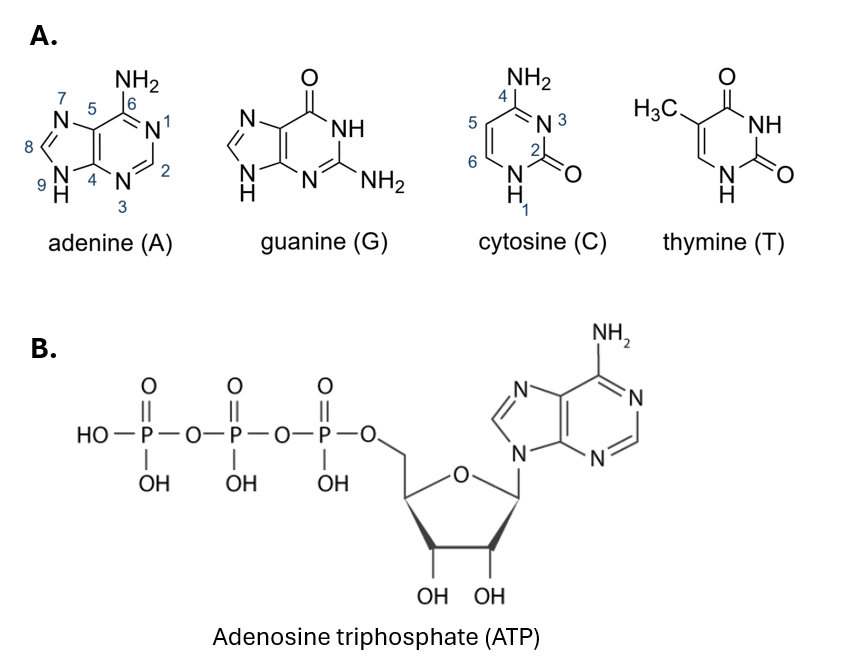
\includegraphics[scale=.8]{Picture10}\\
\caption{A) Chemical structures of the DNA bases. B) ATP: one of the four nucleotides of DNA and a primary energy unit in most organisms.}
\end{figure}

\begin{figure}[H]
\centering
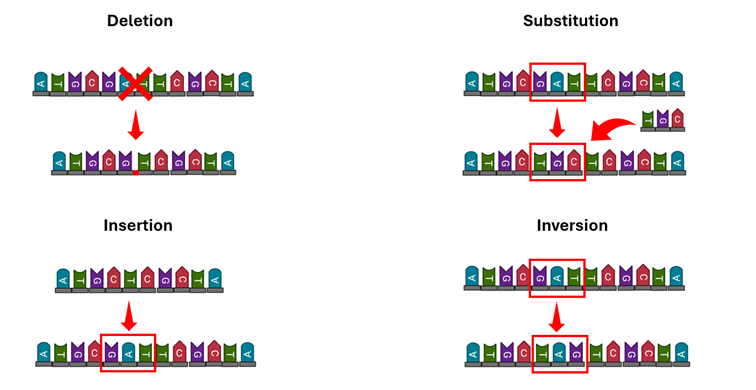
\includegraphics[scale=1]{Picture4}\\
\caption{Different types of Mutation at the DNA level. created by https:/www.biorender.com}
\end{figure}



\section{Genetic Algorithms}

Genetic Algorithms are a family of computational models inspired by biological evolution. They are used to solve problems heuristically by utilizing fundamental concepts of evolution. Any possible solution to a specific problem is called a chromosome or individual, and a population is the pool of solutions related to that specific problem.

In the first step of these algorithms, all individuals are evaluated by a specific fitness function. This function allows us to rank the solutions based on their effectiveness, giving higher chances to those chromosomes that offer better solutions to the problem. This process of grading and assigning higher probabilities to better solutions simulates natural selection. In nature, individuals in a species that are better adapted and carry advantageous genes have a higher chance of passing those genes to their offspring.

Next, using fundamental concepts of evolution like recombination (crossover) and mutation, the chromosomes are altered to create better solutions for the problem. The modified chromosomes are then sent to the next generation. This process is repeated over multiple iterations until the algorithm converges to an optimal or near-optimal solution. These algorithms belong to the optimizer family and are typically used to improve the population iteratively, aiming for a better approximation or sometimes the exact solution to the problem.\\[6px]

\begin{figure}[H]
\centering
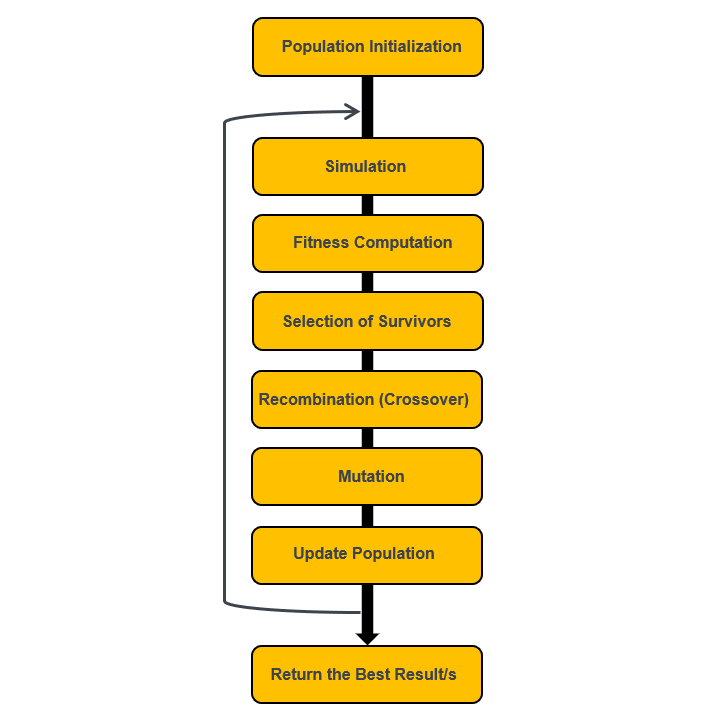
\includegraphics[scale=.7]{Picture11}\\
\caption{Illustration of the fundamental of Genetic Algorithms}
\end{figure}



\subsection{Natural Selection}

In nature, individuals with favorable traits have a better chance of surviving and adapting to their environment. They also have a higher likelihood of producing offspring that inherit these advantageous genes, shaping the gene pool of future generations through a process known as natural selection.

To simulate a genetic algorithm on a computer and harness the power of natural selection to solve a problem, the first step is to define a finite population (listing 1). This population consists of individuals (chromosomes) that represent possible solutions to the problem. These individuals can be initialized using random sampling or other methods that ensure a diverse distribution of potential solutions.

The next critical step is to define a fitness function (similar to a cost function in machine learning models) that evaluates each individual based on how well it solves the problem. The fitness function assigns a numerical score to each individual, reflecting its effectiveness as a solution. Individuals with higher fitness scores are considered to offer better solutions to the problem.

The algorithm then uses these fitness scores to select individuals for reproduction, mimicking natural selection. Individuals with higher fitness scores have a greater probability of being selected to produce offspring and contribute to the gene pool of the next generation. This iterative process, where individuals with better solutions are more likely to pass on their genes, mirrors the concept of artificial natural selection applied to a population of solutions.



\begin{lstlisting}[language=Python, caption={Initialize a population for a genetic algorithm}, numbers=none, breaklines=true]
def initialize_population(pop_size, bit_length):

    """
    Initialize a population for a genetic algorithm.

    Args:
        - pop_size (int): The number of individuals in the population.
        - bit_length (int): The length of the binary string representing each individual.

    Returns:
        - population (list): A list of binary strings, each representing an individual in the population.
    """
    population = [
        ''.join(random.choice('01') for _ in range(bit_length)) for _ in range(pop_size)
        ]    
    return population  
\end{lstlisting}


\subsection{Fitness Function}

In biology, fitness refers to the quantitative measure of an individual's reproductive success, or more specifically, a chromosome's ability to contribute offspring to the next generation. In genetic algorithms, the fitness function serves as a measure of the reproductive success of a solution or chromosome, which should be maximized. This means individuals with higher fitness values have a greater chance of being selected for further exploration during the optimization process.

Choosing an appropriate fitness function depends on the characteristics of the population and the nature of the problem being addressed. For maximization problems, the fitness function directly corresponds to the objective function (listing 2), denoted as ${F(i) = O(i)}$. However, for minimization problems, the objective function needs to be transformed to align with the maximization goal of the fitness function.


One common transformation for minimization problems is:

$$F(x) = \frac{1}{1 + f(x)}$$

Here, $f(x)$ represents the objective function to be minimized. This transformation ensures that higher values of $f(x)$ result in higher fitness values $F(x)$, effectively turning a minimization problem into a maximization one without changing the locations of individual fitness values.


Another approach to transform the objective function for minimization problems is:

$$F(i) = V - \frac{O(i).P}{\sum_{i=1}^p O(i)}$$

In this transformation, $O(i)$ represents the objective function value of the $i$-th individual, PP denotes the population size, and $V$ is a sufficiently large value to ensure non-negative fitness values. This formula redistributes the fitness values such that individuals with lower objective function values (indicating better solutions in minimization problems) receive higher fitness scores.

These transformations enable genetic algorithms to effectively handle both maximization and minimization problems by appropriately aligning the fitness function with the objectives of the optimization process.\\[6px]


\begin{lstlisting}[language=Python, caption={Fitness Function}, numbers=none, breaklines=true]

def compute_fitness(population, target):
    """
    Compute the fitness value for each individual in the population.

    Args:
        population (list of str): The population of individuals, each represented as a binary string.
        target (str): The target binary string to compare against.

    Returns:
        fitness_values (list of int): A list of fitness values, one for each individual in the population.
    """
    fitness_values = []

    for individual in population:
        fitness = sum(1 for i, j in zip(individual, target) if i == j)
        fitness_values.append(fitness)

    return fitness_values
    
\end{lstlisting}





\subsection{Genetic Algorithm Operators}

In genetic algorithms, there are three primary operators: reproduction, recombination (crossover), and mutation. Each individual or chromosome in the population represents a solution to the problem at hand. These individuals are evaluated based on their fitness, combined, altered, and modified through crossover and mutation to create a new population. This iterative process continues until termination criteria are met.

One complete cycle of this operation, including fitness evaluation, selection, and modification (via recombination and mutation), is termed a generation in genetic algorithm terminology.


\subsubsection{Selection of Survivors}

After evaluating all individuals in the randomly generated population, either directly by comparing each individual's fitness or indirectly, such as in simulation tasks where outputs are evaluated against targets, the next step in the genetic algorithm is to generate a new, potentially improved generation from the current one (often the first generation).

To achieve this, individuals from the current population are randomly chosen to populate the new generation. Each individual is assigned a weight based on its fitness: higher fitness results in a higher weight. The probability of each individual being selected for the next generation is directly proportional to its weight. For example, if individual $X$ has a weight of $0.8$ and individual $Y$ a weight of $0.4$, then individual $X$ has twice the chance of being selected for the next generation compared to individual $Y$.

This selection method is commonly known as Roulette Wheel Selection (listing 3). Mathematically, the probability $p_i$ of selecting the $i$-th individual to be part of the next generation is calculated as:

$$p_{i} = \frac{f_i}{\sum_{i=1}^{n}f_i}$$


where $n$ is the population size, $p_i$ is the probability for the $i$-th individual, and $f_i$ is the fitness value of the $i$-th individual.

To visualize this method, imagine a roulette wheel divided into segments proportional to each individual's fitness or weight. The wheel is spun $n$ times, and each spin randomly selects an individual based on its segment size, determined by the calculated probabilities. Figure 7 provides a schematic representation of this selection process.

This method of survivor selection ensures that individuals with higher fitness contribute more significantly to the next generation, allowing genetic algorithms to iteratively improve solutions over successive generations.


\begin{figure}[H]
\centering
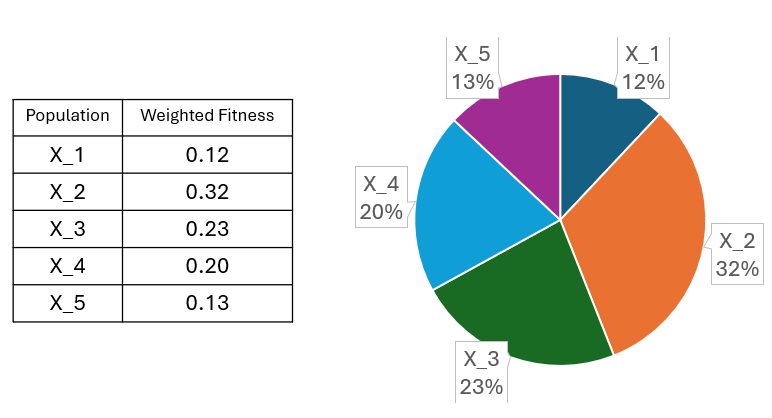
\includegraphics[scale=1]{Picture6}\\
\caption{A roulette-wheel marked for five individuals according to their fitness values.}
\end{figure}


\begin{lstlisting}[language=Python, caption={Roulette Wheel Selection}, numbers=none, breaklines=true]

def select_parents_roulette(population, fitness_scores, population_size):
    """
    Select parents for the next generation based on their fitness scores
    using the Fitness Proportionate Selection (Roulette Wheel Selection) method.

    Args:
        population (list of str): The current population of individuals, each represented as a binary string.
        fitness_scores (list of int): The fitness scores of the individuals in the population.
        population_size (int): number of chromosomes in the original population

    Returns:
        selected (list): The selected parents for the next generation.
    """

    total_fitness = np.sum(fitness_scores)

    if total_fitness == 0:
        probabilities = np.ones(len(fitness_scores)) / len(fitness_scores)
    else:
        probabilities = np.array(fitness_scores) / total_fitness

    selected_indices = np.random.choice(len(population), size=population_size, p=probabilities)
    selected = [population[i] for i in selected_indices]

    return selected 
    
\end{lstlisting}




\subsubsection{Recombination (Crossover)}

In the crossover process (listing 4)of genetic algorithms, the objective is to create new and potentially improved individuals (chromosomes) by combining information from two parent chromosomes. Two parent chromosomes are selected from the previous generation. A randomly chosen index determines where the exchange of genetic material will occur between the parents. Typically, one part of a chromosome from one parent (before the index) is swapped with the corresponding part of the other parent (after the index), resulting in two offspring chromosomes.

Figure 8 illustrates how this crossover process generates new chromosomes from six parent chromosomes encoded with binary representations. It shows examples of both one-point crossover and two-point crossover mechanisms.



The effectiveness of crossover can vary, it may or may not lead to beneficial outcomes. To preserve some of the well-performing chromosomes (those with relatively high fitness) without alterations, a crossover rate is introduced. This rate determines the proportion of parent pairs that undergo crossover to produce offspring, while the remaining individuals are directly passed on to the next generation unchanged.

The primary goal of crossover is to exchange genetic information between chromosomes to potentially create offspring that are better adapted to the problem at hand.
 
 
 
\begin{figure}[H]
\centering
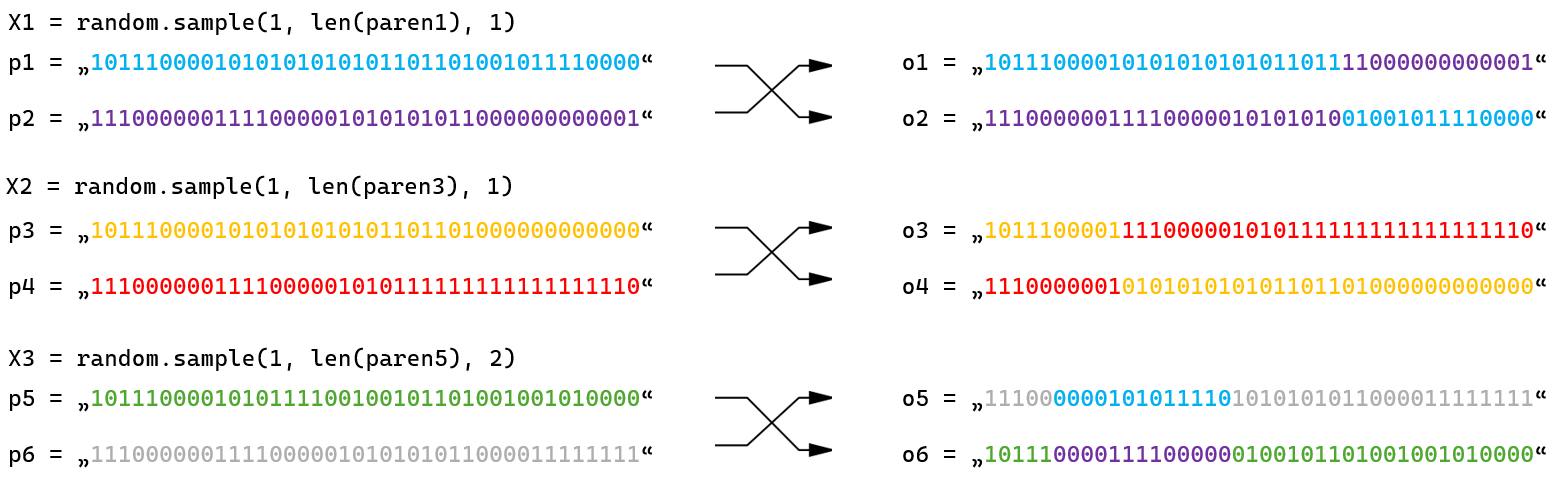
\includegraphics[scale=0.40]{Picture7}\\
\caption{Crossover process between among 6 chromosomes, which are encoded with binary representations. the fist two parent pair went through a one site crossover, while the third pair went through a two site crossover.}
\end{figure}

\newpage


\begin{lstlisting}[language=Python, caption={multi-point crossover}, numbers=none, breaklines=true]

def crossover(parent1, parent2, crossover_rate, num_crossover_points):
    """
    Perform multi-point crossover between two parents to generate two offspring.

    Args:
        parent1 (str): A binary string representing the first parent.
        parent2 (str): A binary string representing the second parent.
        crossover_rate (float): Probability of performing crossover for the chromosome.
        num_crossover_points (int): An integer representing the crossover points for the chromosome.

    Returns:
        tuple: Two binary strings representing the offspring.
    """
    if random.random() < crossover_rate:
        crossover_points = sorted(random.sample(range(1, len(parent1)), num_crossover_points))
        child1, child2 = "", ""
        start = 0

        for i, point in enumerate(crossover_points + [len(parent1)]):
            if i % 2 == 0:
                child1 += parent1[start:point]
                child2 += parent2[start:point]
            else:
                child1 += parent2[start:point]
                child2 += parent1[start:point]
            start = point

        offspring1, offspring2 = child1, child2
    else:
        offspring1, offspring2 = parent1, parent2

    return offspring1, offspring2
    
\end{lstlisting}








\subsubsection{Mutation}

Mutation is a crucial operator in genetic algorithms that introduces random changes in offspring chromosomes after the recombination process, thereby diversifying the population over successive generations (listing 5). Its primary objective is to prevent the algorithm from becoming stuck in local optima by adding new genetic information that may lead to better solutions.

After undergoing the crossover process (as depicted in Figure 8), chromosomes proceed to mutation (as shown in Figure 9). Mutation randomly alters individual bits within chromosomes with a small probability. This random disturbance affects the genetic information stored in each chromosome, contributing to the generation of diverse solutions.

Figure 9 illustrates the mutation process occurring in the six chromosomes that underwent the crossover process (Figure 8). Each chromosome undergoes random bit flips, ensuring that the genetic diversity necessary for the evolutionary process is maintained over iterations.


\begin{figure}[H]
\centering
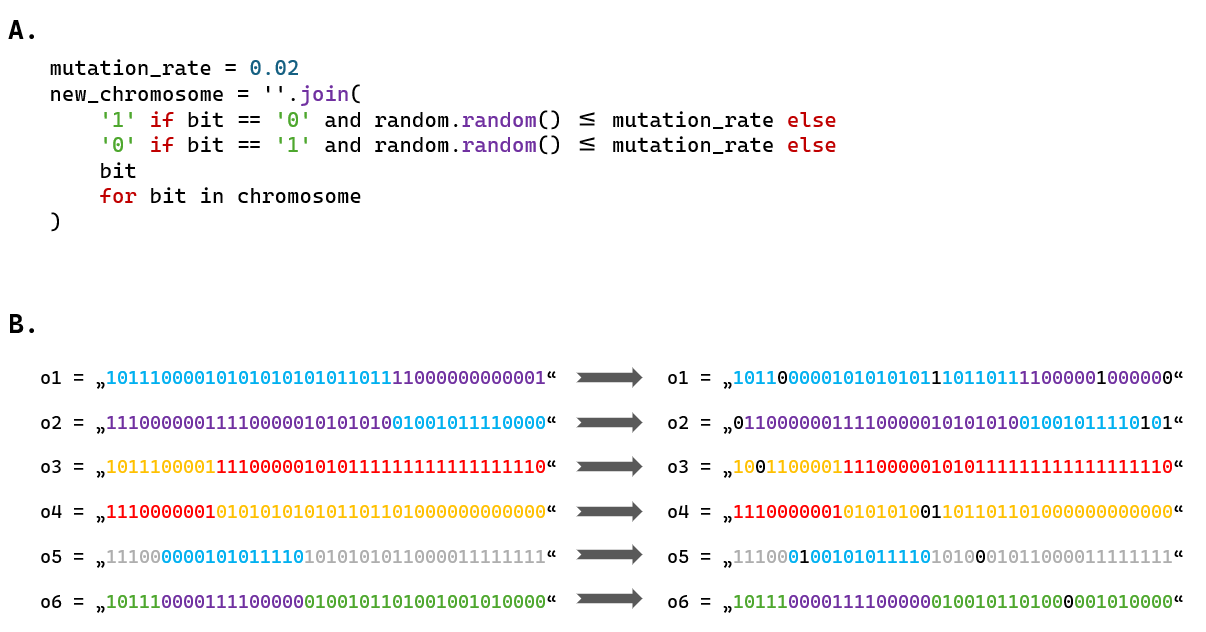
\includegraphics[scale=0.60]{Picture8}\\
\caption{Mutation process. A) the python code to change the bits in a chromosome based on the mutation probability. B) the six chromosomes after crossover in the previous part which are going to change their information with mutation process.}
\end{figure}


\newpage


\begin{lstlisting}[language=Python, caption={Mutate a chromosome  based on its mutation rate}, numbers=none, breaklines=true]

def mutate(chromosome, mutation_rate):

    """
    Mutate a chromosome  based on its mutation rate.

    Args:
        - chromosome (str): a binary strings representing the chromosome,
        - mutation_rate (float): The probability of mutating each bit in chromosome.

    Returns:
        - mutated_chromosome (str): The mutated chromosome

    Example:
        chromosome = '100001110010101010110'
        mutation_rate = 0.1
        mutated_chromosome = mutate(chromosome, mutation_rates)
    """
    mutated_chromosome = ''.join(
        '1' if bit == '0' and random.random() <= mutation_rate else
        '0' if bit == '1' and random.random() <= mutation_rate else
        bit
        for bit in chromosome
    )

    return mutated_chromosome
    
\end{lstlisting}



\subsection{Optimization}

After generating the next generation (as indicated in the "update population" block in Figure 6), each individual, chromosome, in the new generation is evaluated. This process is repeated iteratively until one or more individuals in the population achieve the highest possible fitness. These individuals are then chosen as the best possible solutions for the problem.

In some cases, a threshold for the highest fitness can be defined, allowing the algorithm to terminate early when this threshold is reached or exceeded.

Now, we can put all these concepts together and create the complete genetic algorithm, which we will use to solve some basic optimization problems. In the code block below (listing 6), there are three functions: the main function named genetic-algorithm, which orchestrates the process by calling other functions in the correct order (as described in Figure 6), and two helper functions (extract-based-on-max-index and decimal-to-binary), which are utilized by the main function.


\newpage
\begin{lstlisting}[language=Python, caption={Genetic Algorithm}, numbers=none, breaklines=true]

def genetic_algorithm(population_size, mutation_rate, crossover_rate, num_crossover_points,
                      target, precision_bits, max_generation=1000, fitness_trigger=None):

    """
    Execute a genetic algorithm to optimize a population of binary-encoded chromosomes.

    Args:
        population_size (int): Number of individuals in the population.

        component of the chromosomes. (min_val, max_val, bits)
        max_generation (int): maximum Number of generations to run the algorithm.
        mutation_rate (float): Probability of mutating each bit in each chromosome.
        crossover_rate (float): Probability of performing crossover for each chromosome.
        num_crossover_points (int): number of crossover points in chromosome.
        target (numpy.ndarray): Target array to compare simulation results against.
        precision_bits (tuple): Tuple containing (min_val, max_val, bits) for encoding the target.
            - min_val (float): Minimum possible value of the target range.
            - max_val (float): Maximum possible value of the target range.
            - bits (int): Number of bits used to represent the target values in the binary string.

        fitness_trigger (int or float): fitness threshold to break the algorithm

    Returns:
        population (list): Final population of binary-encoded chromosomes.
    """

    elite_chromosomes = []  # list to store the best binary chromosome of each generation
    best_fitness = []  # list to store the best fitness of each generation

    print(f"{'-' * 40}")
    print("      *** Genetic Algorithm *** ")
    print(f"{'-' * 40}")

    binary_target = decimal_to_binary(array=target, precision_bits=precision_bits)
    population = initialize_population(
        pop_size=population_size,
        bit_length=len(binary_target)
    )


    if fitness_trigger:
        max_fitness = fitness_trigger
    else:
        max_fitness = len(binary_target)

    max_generation_fitness = 0
    generation = 1

    while generation <= max_generation and max_generation_fitness < max_fitness:

        generation_fitness = compute_fitness(
            population=population,
            target=binary_target
        )

        elite_chromosomes.append(extract_based_on_max_index(list1=population, list2=generation_fitness))
        max_generation_fitness = max(generation_fitness)
        best_fitness.append(max_generation_fitness)

        if max_generation_fitness == max_fitness:
            print()
            print("The Algorithm Found The Best Solution (max fitness == max generation fitness)")
            break

        new_population = []
        parents = select_parents_roulette(
            population=population,
            fitness_scores=generation_fitness,
            population_size=population_size
        )

        for _ in range(len(parents) // 2):

            while len(parents) >= 2:
                parent1 = random.choice(parents)
                parents.remove(parent1)

                if len(parents) > 0:
                    parent2 = random.choice(parents)
                    parents.remove(parent2)
                else:
                    parent2 = parent1
                break  # Exit the while loop after selecting parent1 and parent2

            offspring1, offspring2 = crossover(
                parent1=parent1,
                parent2=parent2,
                crossover_rate=crossover_rate,
                num_crossover_points=num_crossover_points
            )
            new_population.extend([
                mutate(
                    chromosome=offspring1,
                    mutation_rate=mutation_rate
                ),
                mutate(
                    chromosome=offspring2,
                    mutation_rate=mutation_rate
                )
            ])

        print(f"Generation {generation}; Best/Max Fitness: {max_generation_fitness}/{max_fitness}")
        population = new_population
        generation += 1

    average_fitness = sum(best_fitness) / len(best_fitness)

    print(f"{'------------------------------------------'}")
    print(f"      Simulation Complete!")
    print(f"      The best found fitness: {max(best_fitness)}")
    print(f"      Total Generations: {len(best_fitness)}")
    print(f"      Average Fitness: {average_fitness:.2f}")
    print(f"{'------------------------------------------'}")

    return (population, elite_chromosomes, best_fitness, generation)
    
 
def extract_based_on_max_index(list1, list2):
    """
    Extract an object from list1 based on the index of the maximum value in list2.

    Args:
        list1 (list): The list from which to extract the object.
        list2 (list): The list used to determine the index of the maximum value.

    Returns:
        object: The object from list1 corresponding to the index of the maximum value in list2.
    """
    max_index = list2.index(max(list2))

    return list1[max_index]
    


def decimal_to_binary(array, precision_bits):
    """
    Convert a  NumPy array to a binary string.

    Args:
        - array (numpy.ndarray): an arrays of float or int values.
        - precision_bits (tuple): tuple containing (min_val, max_val, bits) to define the precision for array.
            - min_val (float): The minimum possible value of the original range for the element.
            - max_val (float): The maximum possible value of the original range for the element.
            - bits (int): The number of bits used to represent the element in the binary string.

    Returns:
        - binary_string (str): a binary string representing the array.
    """

    min_val, max_val, bits = precision_bits

    if max_val == min_val:
        # All values will be the same in this case, handle gracefully by converting to '0' * bits
        binary_string = ''.join(
            '0' * bits
            for _ in array
        )
    else:
        binary_string = ''.join(
            f"{int((val - min_val) / (max_val - min_val) * ((1 << bits) - 1)):0{bits}b}"
            if not np.isnan(val) else '0' * bits  # Handle NaN by converting to '0' * bits
            for val in array
        )

    return binary_string
    
\end{lstlisting}

\newpage


\section{Application of Genetic Algorithm to Solve a Simple Optimization Problem}

To demonstrate the effectiveness of the genetic algorithm (GA) discussed in this article, we applied it to a simple optimization problem. The problem is to find a specific target binary string of length 48 bits. The goal is to evolve a population of binary strings to match this target string as closely as possible.

\subsection{Experimental Setup}

The GA was run 10 times, each with a maximum of 300 generations. For each generation, the best solution (the one with the highest fitness) was recorded. The fitness function used was a simple matching count, where the fitness score was the number of bits matching the target string.

In another experiment, we analyzed the relationship between the length of the chromosome and the number of generations required to find the optimal solution. The GA was run 9 times, each time with an increasing chromosome length (10, 15, 20, ..., 50) and a maximum of 2000 generations. The best solution of each run was recorded and plotted to visualize the association between chromosome length and the number of generations needed.

\subsection{Results and Analysis}

Figure 10 shows the results of the 10 runs with a chromosome length of 48 bits. Each line represents the highest fitness score achieved in each generation across the 10 runs. As expected, the plot shows a stochastic representation of the system, indicating variability in the performance of the GA due to its inherent randomness. Despite this stochastic behavior, the general trend shows that the fitness scores improve over generations, demonstrating the GA's ability to evolve better solutions over time.

\begin{figure}[H]
\centering
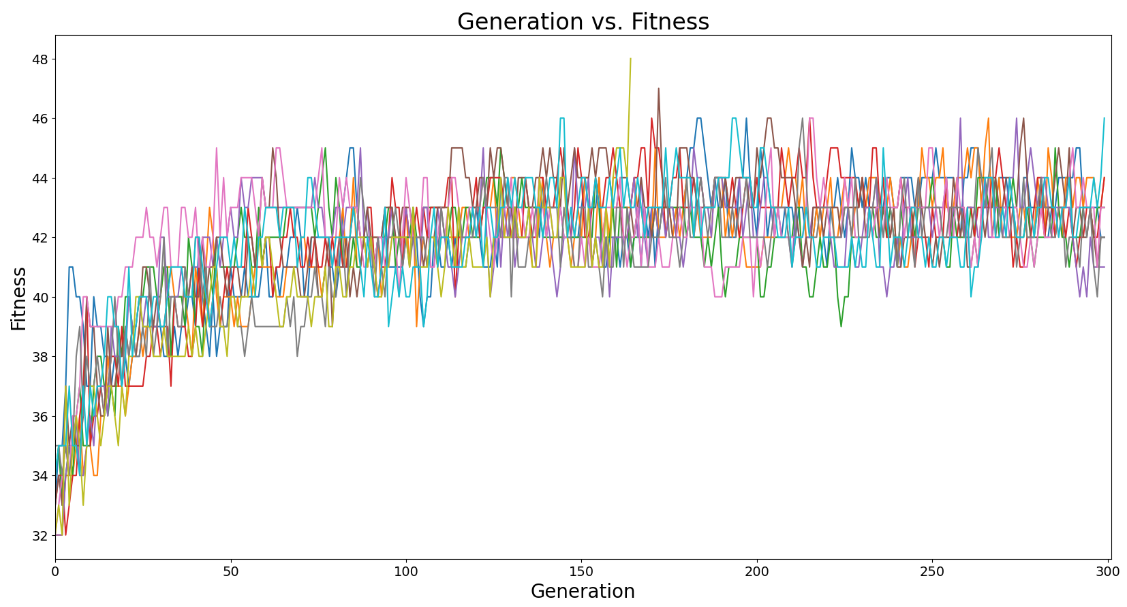
\includegraphics[scale=0.60]{stochastic_effect}\
\caption{Stochastic representation of the genetic algorithm's performance over 10 runs with a chromosome length of 48 bits. Each line represents the highest fitness score achieved in each generation.}
\end{figure}

Figure 11 illustrates the relationship between chromosome length and the number of generations needed to find the optimal solution. As the chromosome length increases, the number of generations required to achieve the highest fitness score also increases. This relationship appears to be exponential, indicating that longer chromosomes require significantly more generations to evolve to the optimal solution. This result is consistent with the expectation that as the search space increases, the GA requires more iterations to explore and find the best solution.

\begin{figure}[H]
\centering
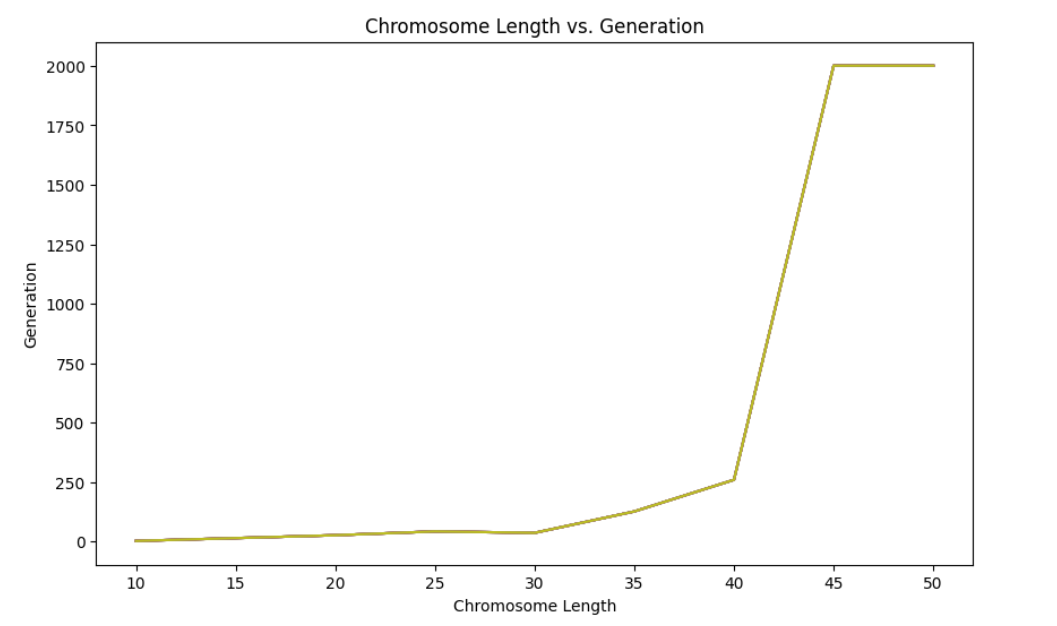
\includegraphics[scale=0.60]{chr_len}\
\caption{The relationship between chromosome length and the number of generations required to achieve the highest fitness score. The plot shows an exponential increase in the number of generations needed as the chromosome length increases.}
\end{figure}

\subsection{Discussion}

The experiments clearly demonstrate the effectiveness of the GA in optimizing a population of solutions to match a target binary string. The stochastic nature of the results highlights the importance of running the algorithm multiple times to ensure a reliable outcome. Additionally, the exponential relationship between chromosome length and the number of generations needed underscores the challenge of optimizing longer chromosomes and the importance of efficient GA design and parameter tuning.

Overall, these results validate the GA as a powerful optimization tool capable of solving complex problems, albeit with considerations for its stochastic nature and the computational effort required for larger problem spaces.


 

\section{Conclusion}

Genetic algorithms harness the principles of natural selection to solve complex optimization problems. Inspired by biological evolution, these algorithms iterate through generations of potential solutions, using selection, crossover, and mutation to evolve towards optimal or near-optimal solutions. By simulating the survival of the fittest among a population of solutions, genetic algorithms prove effective in diverse problem domains, from binary string matching to more intricate real-world applications. Their ability to balance exploration and exploitation makes them a valuable tool for tackling problems where traditional methods may fall short. As we continue to refine these algorithms, they promise to play an increasingly significant role in solving complex computational challenges.

\newpage

\section{References}


\href{https://github.com/LoqmanSamani/genetic_algorithms}{GitHub/LoqmanSamani}


\href{http://datajobstest.com/data-science-repo/Genetic-Algorithm-Guide-[Tom-Mathew].pdf}{Genetic Algorithm}



\href{https://www.amazon.de/-/en/Bruce-Alberts/dp/0393884856}{Molecular Biology of the Cell}


\href{https://scholar.google.com/scholar?hl=en&as_sdt=0\%2C5&q=A+Study+on+Genetic+Algorithm+and+its+Applications+L.+Haldurai&btnG=}{A Study on Genetic Algorithm and its Applications}

\href{https://scholar.google.com/scholar?hl=en&as_sdt=0\%2C5&q=Genetic+Algorithm\%3A+Reviews\%2C+Implementations\%2C+and+Applications+Tanweer+Alam&btnG=}{Genetic Algorithm: Reviews, Implementations, and Applications}

\href{https://scholar.google.com/scholar?hl=en&as_sdt=0\%2C5&q=Genetic+Algorithm-+A+Literature+Review+Annu+Lambora\%2C+Kunal+Gupta\%2C+Kriti+Chopra&btnG=}{Genetic Algorithm- A Literature Review}



\end{document}